\subsection{Combined Domain}
We now define a \textit{combined domain} of a given sensitive abstract
domain with the sealed symbolic domain and its one-step execution.
\begin{definition}[Combined Domain]
  A \textit{combined domain} is $\combdom = \sabsdom \times \symbdom$ and its
  concretization function $\combgamma: \combdom \rightarrow \dom$ and join
  operator are defined as follows:
  \begin{align}
    \combgamma((\sabselem, \symbelem)) &= \sgamma(\sabselem) \cup
      \symbgamma(\symbelem)\\
    (\sabselem, \symbelem) \join ({\sabselem}', \symbelem') &= (\sabselem \join
      {\sabselem}', \symbelem \cup \symbelem')
  \end{align}
\end{definition}

Before defining the one-step execution for the combined domain, we introduce
\textit{analysis elements} to easily configure different types of abstract
states in the sensitive abstract domain and the sealed symbolic domain.
\begin{definition}[Analysis Elements]\label{def:aelem}
  An \textit{analysis element} $\aelem \in \aelemset = (\viewset \times \absdom)
  \uplus (\absimapset \times \symbstset)$ is either 1) a pair of a view and an
  abstract state in a sensitive abstract domain $\sabsdom$, or 2) a pair of an
  abstract instantiation map and a sealed symbolic state in a sealed symbolic
  domain $\symbdom$.  Its concretization function $\aelemgamma:
  \aelemset \rightarrow \dom$ is defined as follows:
  \[
    \aelemgamma(\aelem) = \left\{
      \begin{array}{ll}
        \viewmap(\view) \cap \gamma(\abselem) & \text{if} \; (\view, \abselem) = \aelem\\
        \instant{\symbst}{\absimap} & \text{if} \; (\absimap, \symbst) = \aelem\\
      \end{array}
    \right.
  \]
\end{definition}

\begin{figure*}[t]
  \centering
  \begin{subfigure}[t]{0.15\textwidth}
    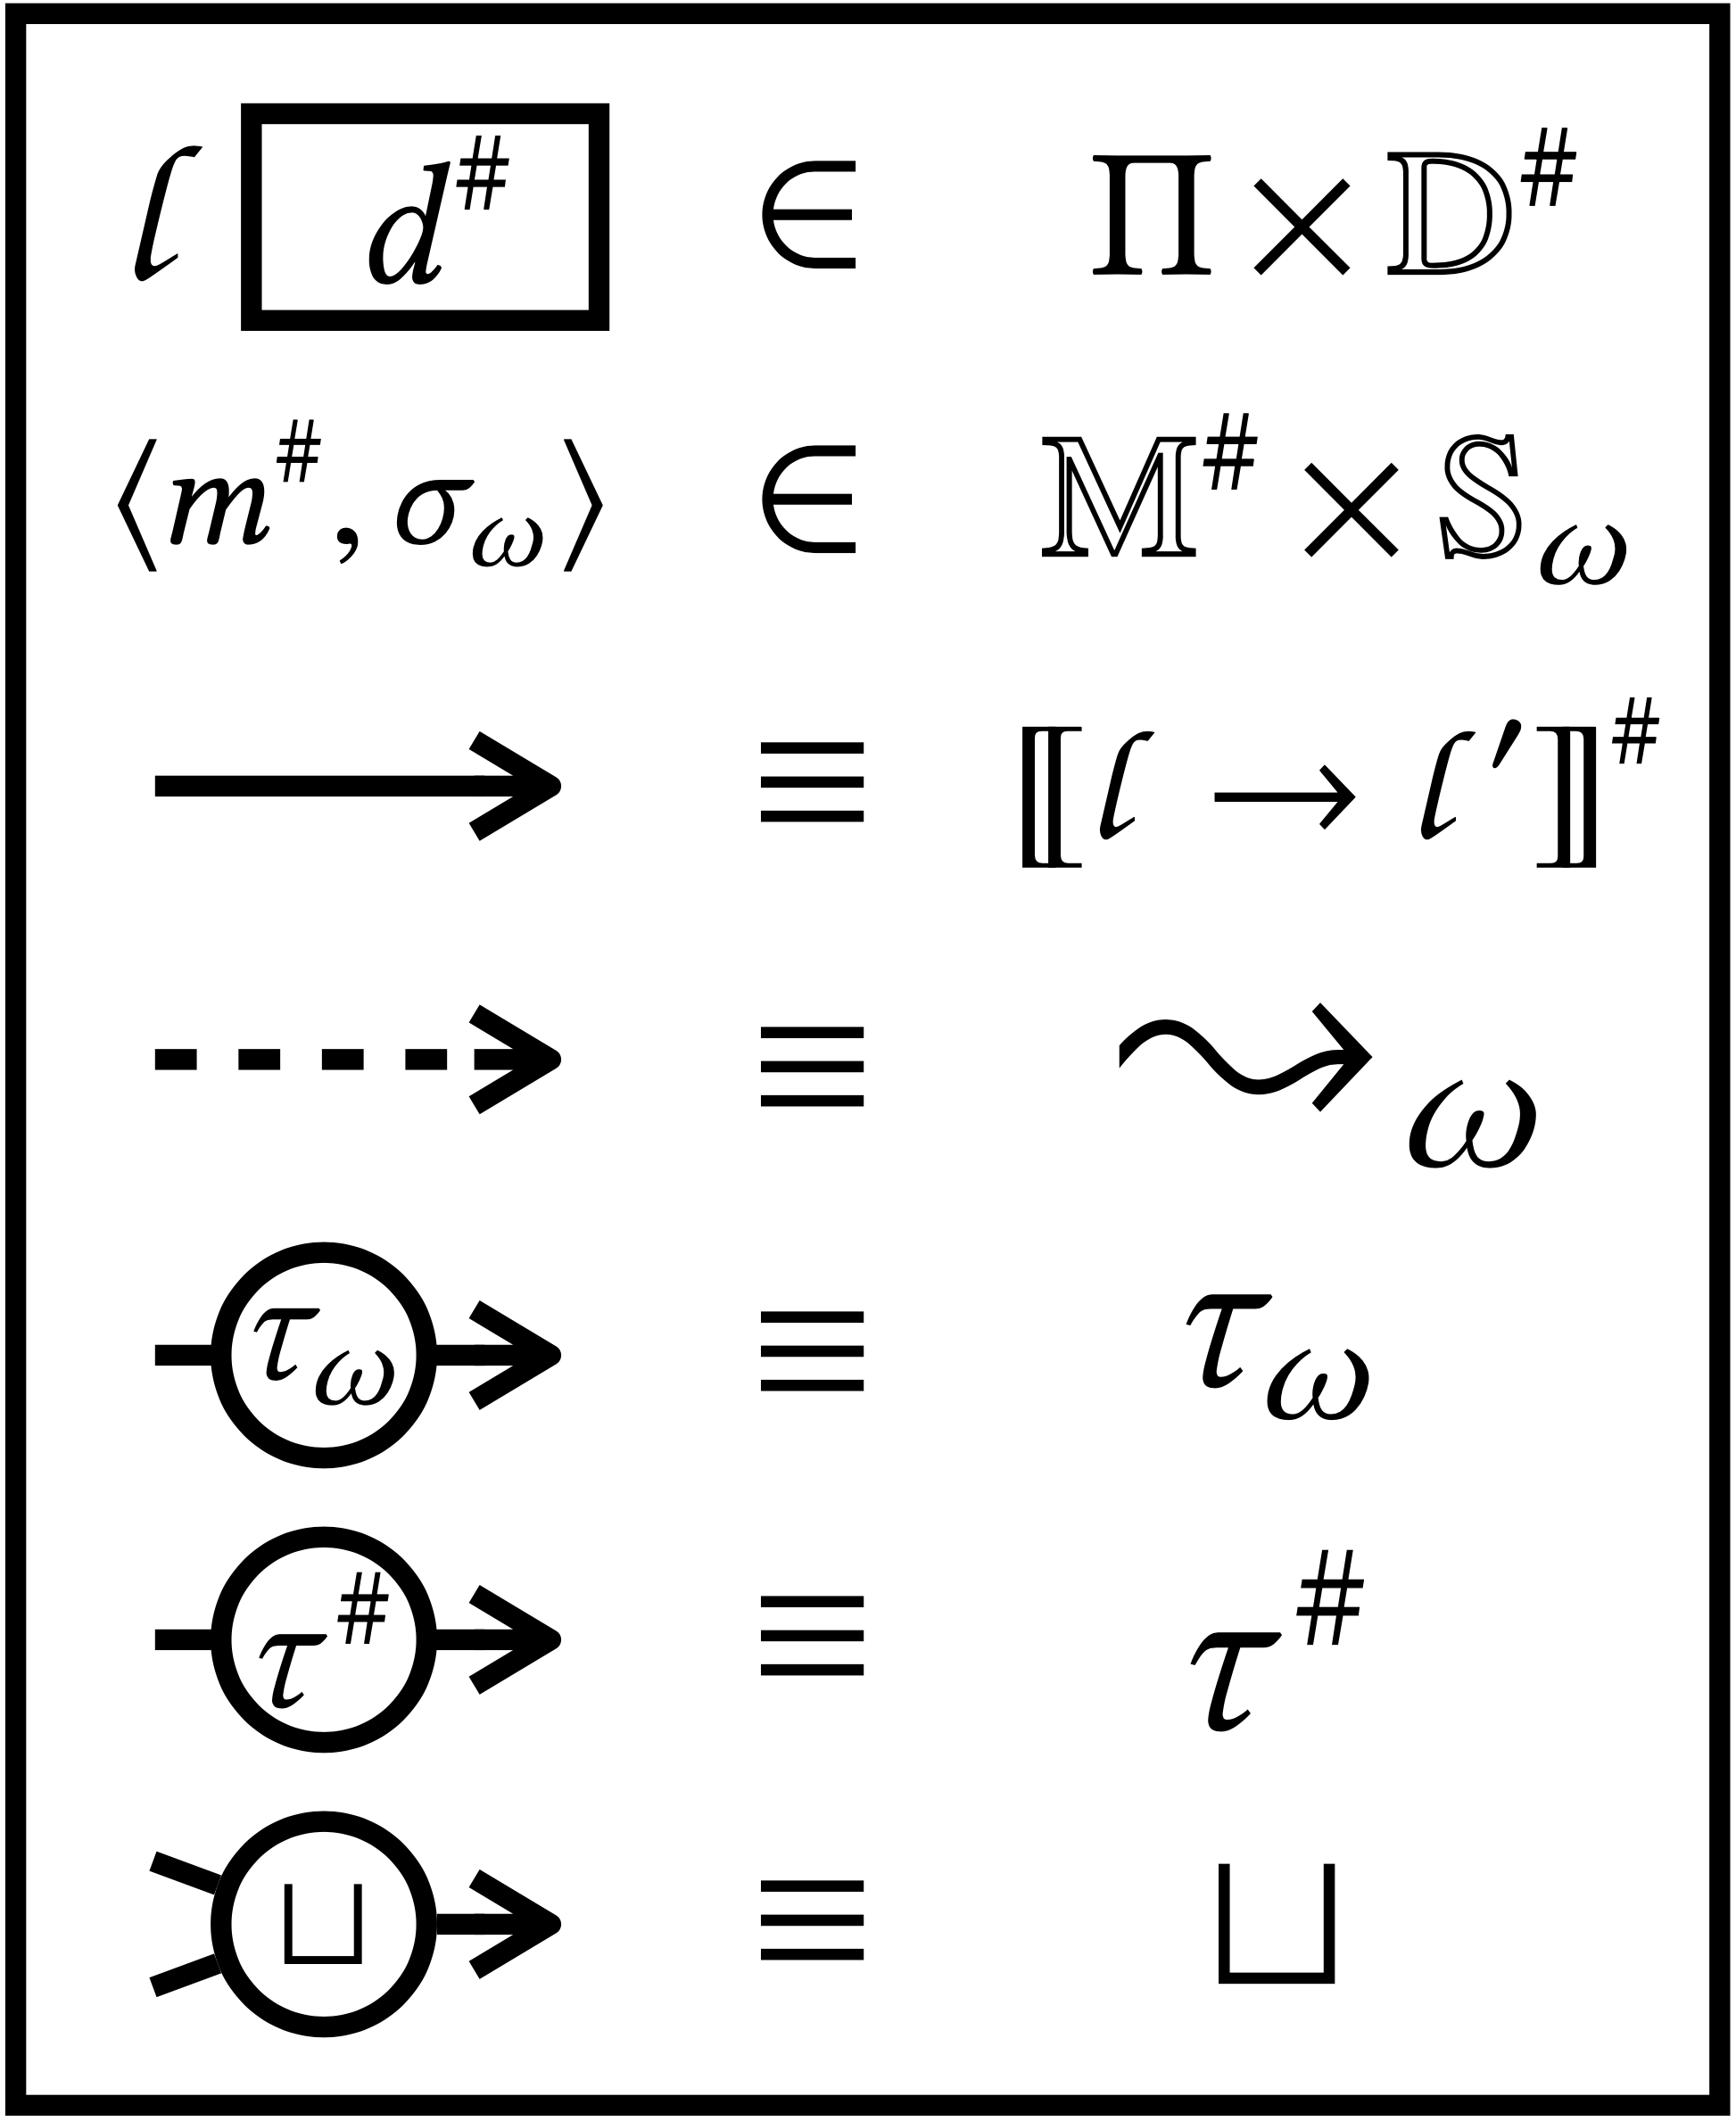
\includegraphics[height=3.2cm]{img/listing}
    \caption{Notations}
    \label{fig:ds-example1}
  \end{subfigure}
  \quad
  \begin{subfigure}[t]{0.23\textwidth}
    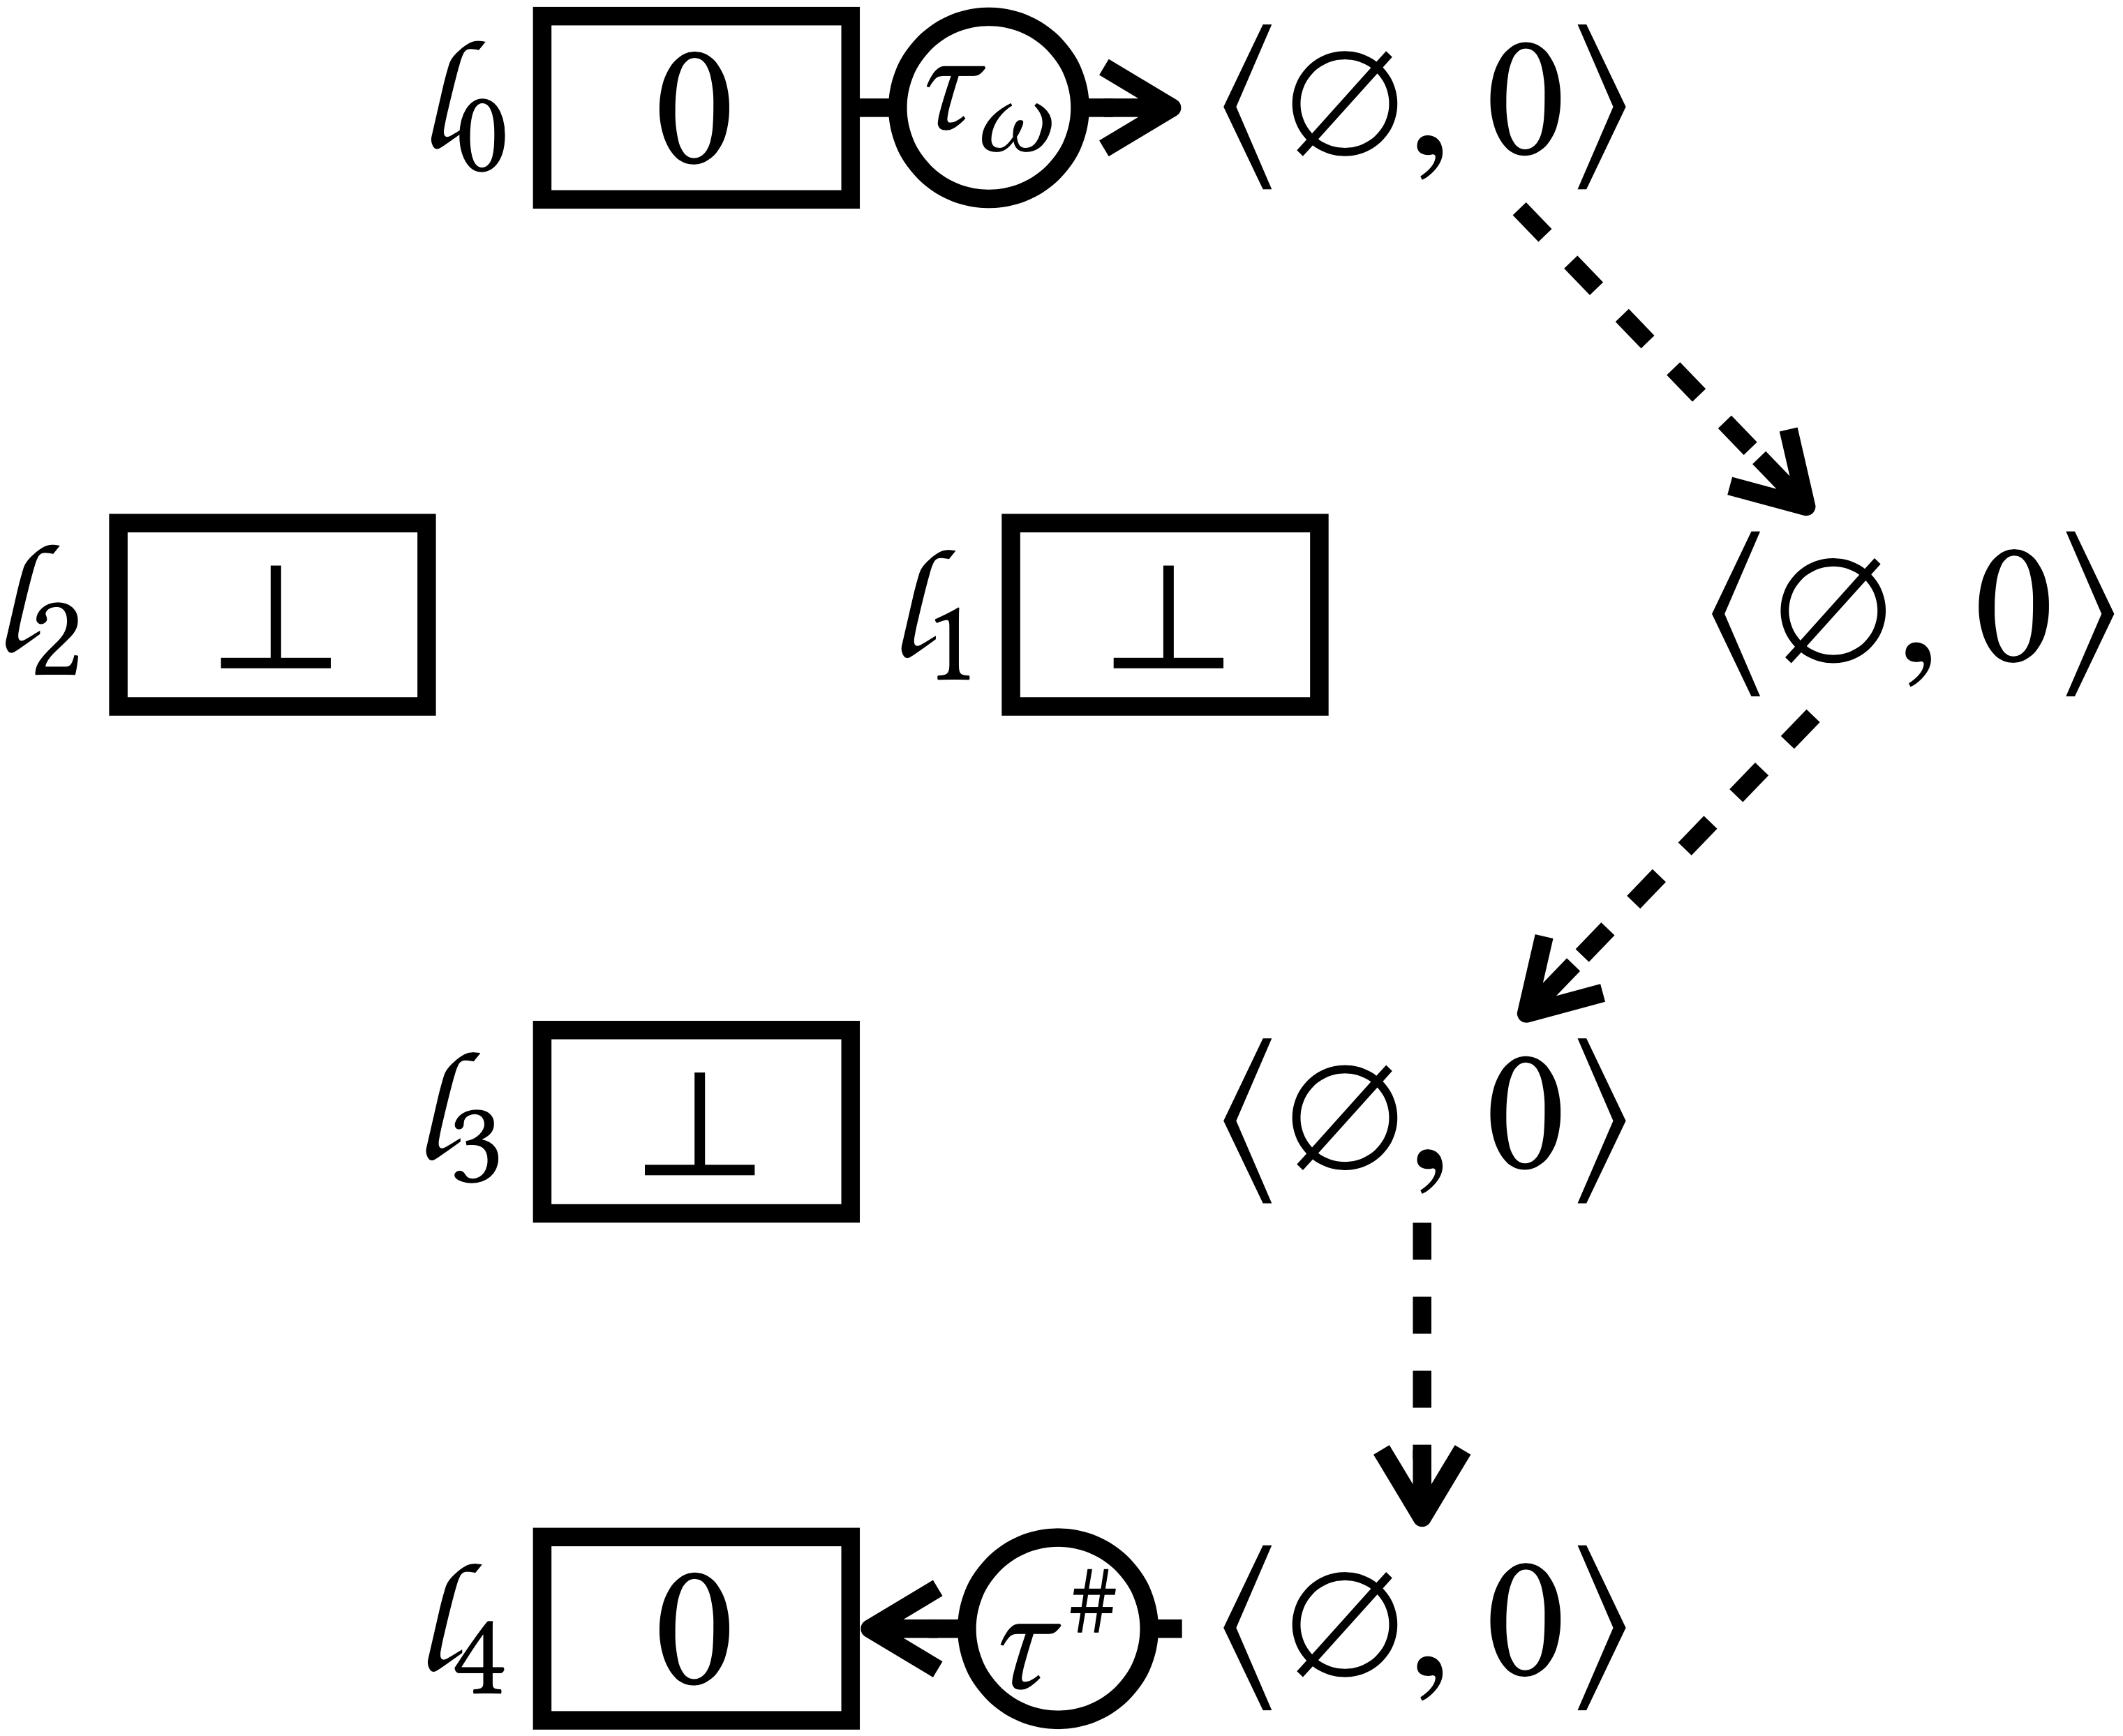
\includegraphics[height=3.2cm]{img/path-1}
    \caption{$\varx = 0$}
    \label{fig:ds-example2}
  \end{subfigure}
  \begin{subfigure}[t]{0.28\textwidth}
    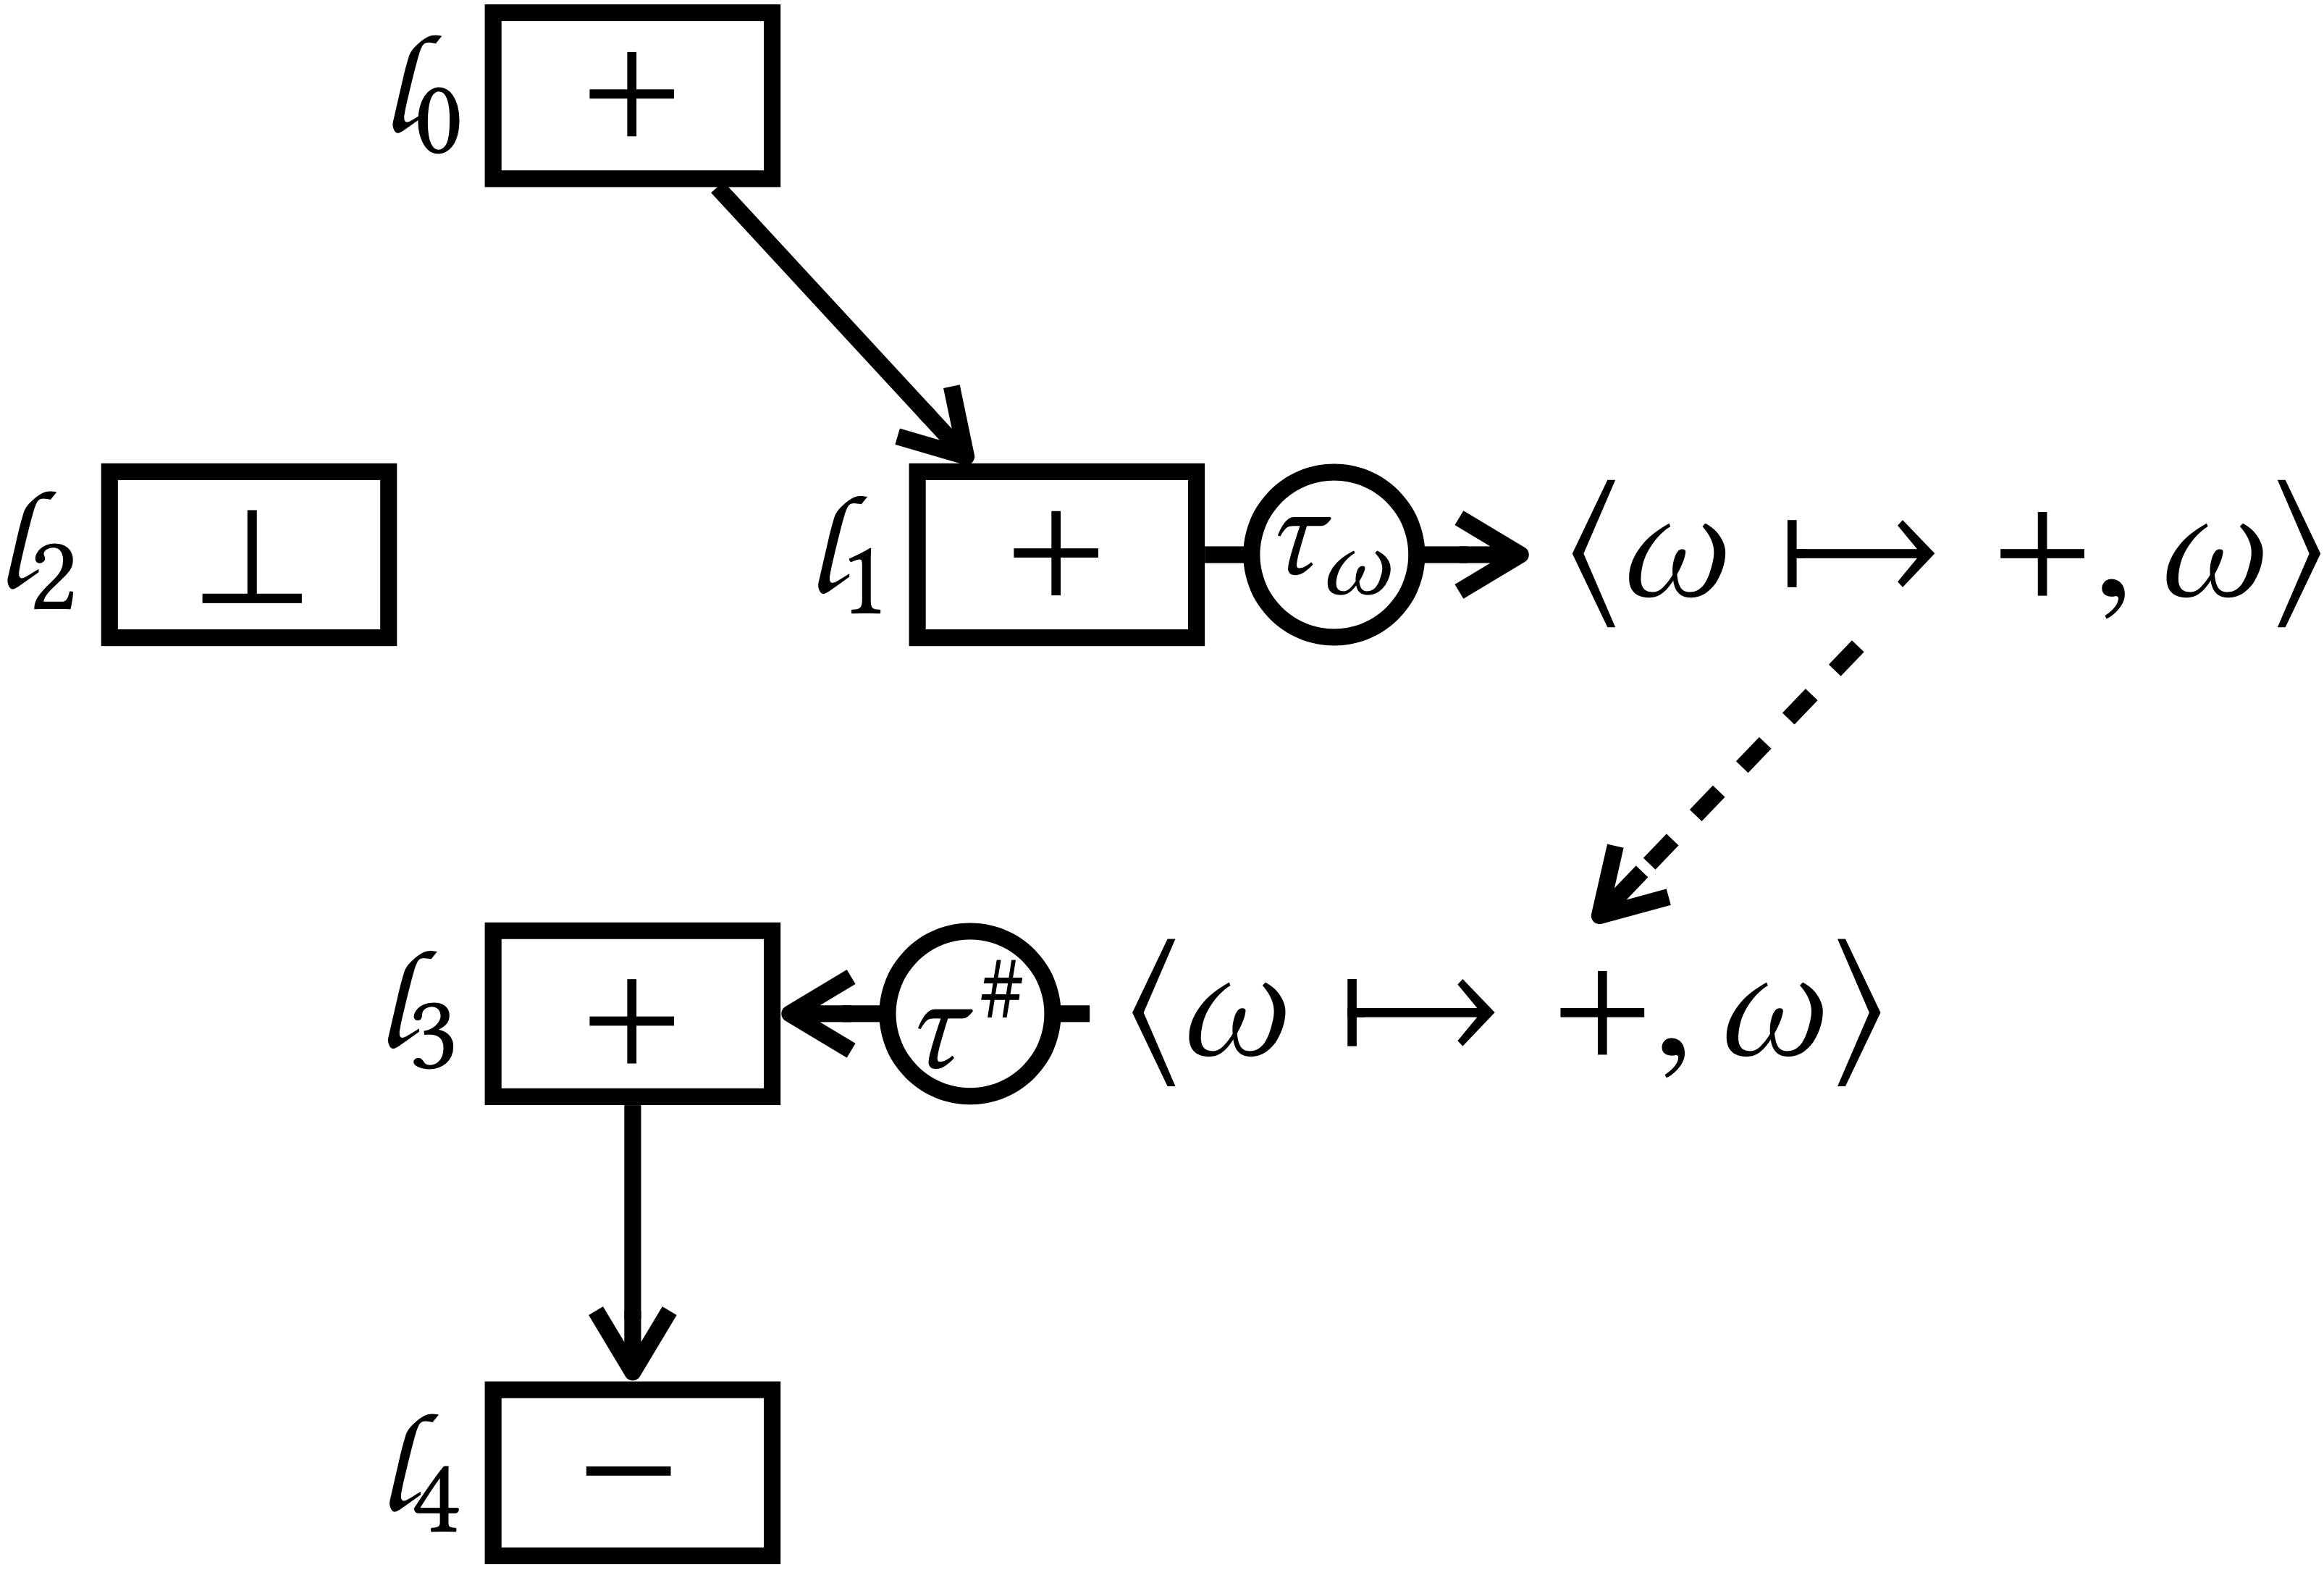
\includegraphics[height=3.2cm]{img/path-2}
    \caption{$\varx > 0$}
    \label{fig:ds-example3}
  \end{subfigure}
  \begin{subfigure}[t]{0.28\textwidth}
    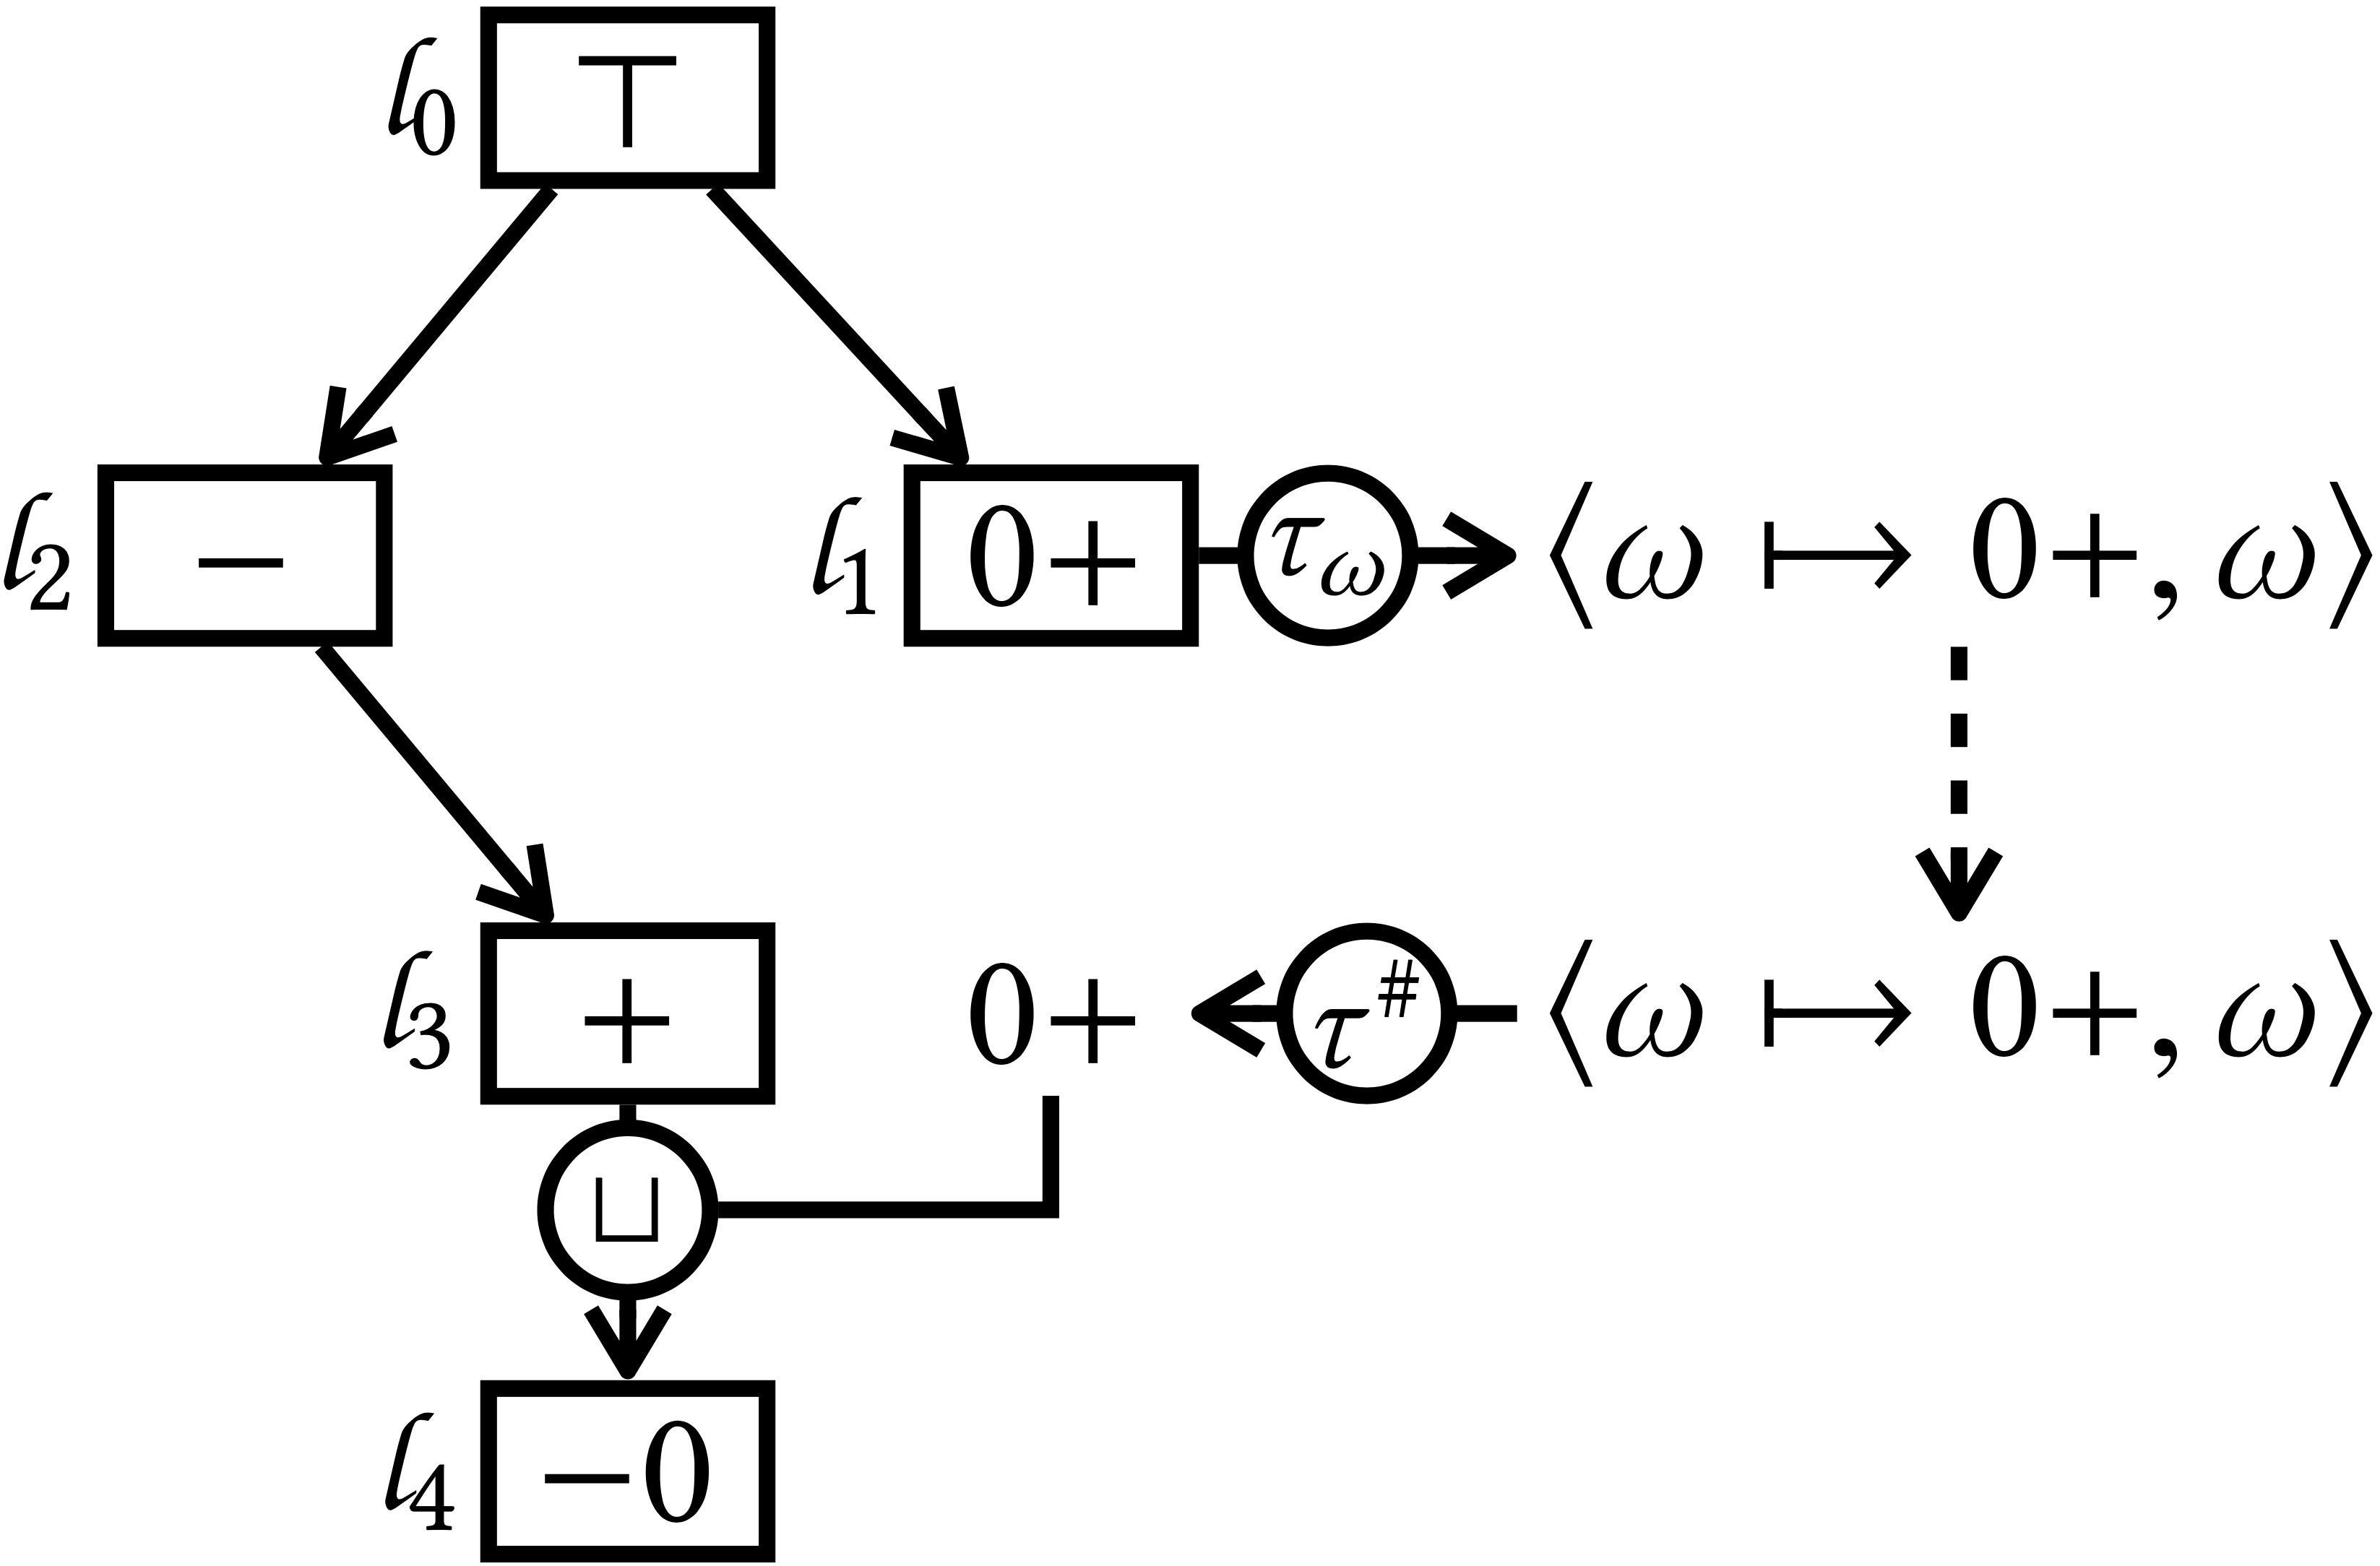
\includegraphics[height=3.2cm]{img/path-3}
    \caption{$\varx \in \mathbb{N}$}
    \label{fig:ds-example4}
  \end{subfigure}
  \caption{Abstract interpretation using a combined domain for the running
  example with different initial values for $\varx$.}
  \label{fig:ds-examples}
\end{figure*}

Moreover, to freely convert between different kinds of analysis elements, we define two converters:
\begin{align}
  \asconverter & : (\viewset \times \absdom) \hookrightarrow
    (\absimapset \times \symbstset)\\
  \saconverter & : (\viewset \times
    \absdom) \leftarrow (\absimapset \times \symbstset)
\end{align}
While the converter $\saconverter$ is total, the other one $\asconverter$ is
\textit{partial}. Thus, it is possible to convert an analysis element
$(\view, \abselem)$ in a sensitive abstract domain to another analysis element in
a sealed symbolic domain only if the convert $\asconverter$ is defined: $(\view,
\abselem) \in \Dom(\asconverter)$.  In addition, they should convert given
analysis elements without loss of information for all $\aelem \in \aelemset$:
\[
  \asconverter(\aelem) = \aelem' \Rightarrow \left\{
  \begin{array}{l}
    \aelem = \saconverter(\aelem')\\
    \aelemgamma(\aelem) = \aelemgamma(\aelem')\\
  \end{array}
  \right.
\]

Now, we define the \textit{combined one-step execution} $\combstep: \combdom
\rightarrow \combdom$ with two converters $\asconverter$ and $\saconverter$.
It consists of two steps: 1) the \textit{\triagename} step converts
analysis elements if a new sealed symbolic execution starts or an
existing one stops, and 2) the \textit{execution} step performs execution of each
analysis element using the abstract one-step execution $\sabsstep$ in the sensitive
abstract domain and the sealed symbolic one-step execution $\symbstep$ in the sealed
symbolic domain.
\begin{definition}[Combined One-Step Execution]
A \textit{combined one-step execution} $\combstep: \combdom \rightarrow
\combdom$ is define as follows:
  \[
    \combstep(\combelem) = (\sabsstep(\sabselem), \symbstep(\symbelem))
  \]
where $(\sabselem, \symbelem) = \triage(\combelem)$.
\end{definition}

From a given combined state $\combelem$, the $\triage$ function makes analysis elements
and converts them if a new sealed symbolic execution
begins or an existing sealed symbolic execution terminates.
Specifically, for an analysis element $(\view, \abselem)$ in the sensitive abstract domain,
if the converter $\asconverter$ is defined for it, $\triage$ introduces a new sealed symbolic execution
by converting the analysis element to its corresponding one $(\absimap, \symbst) =
\asconverter((\view, \abselem))$ in the sealed symbolic domain.
On the other hand, for an analysis element $(\absimap, \symbst)$ in the sealed symbolic domain,
if it does not have any sealed symbolic states to transit to, $\symbst \symbtrans \excst$,
the sealed symbolic execution for $(\absimap, \symbst)$ terminates;
It converts the analysis element to its corresponding one $(\view, \abselem) =
\saconverter((\absimap, \symbst))$ in the sensitive abstract domain and
merges the current abstract state stored in the view $\view$ with $\abselem$.

To formally define the $\triage$ function, we first define a $\atriage$ function
for analysis elements using two converters.
\begin{definition}[$\atriage$]\label{def:atriage}
  The function $\atriage: \aelemset \rightarrow \aelemset$ for analysis elements
  is defined as follows:
  \[
    \atriage(\aelem) = \left\{
      \begin{array}{ll}
        \asconverter(\aelem)
        & \text{if} \; \aelem = (\view, \abselem) \wedge \aelem \in
        \Dom(\asconverter)\\
        \saconverter(\aelem)
        & \text{if} \; \aelem = (\absimap, \symbst) \wedge \symbst \symbtrans
        \bot\\
        \aelem
        & \text{Otherwise}
      \end{array}
    \right.
  \]
\end{definition}
\begin{definition}[$\triage$]\label{def:triage}
  The \triagename function $\triage: \combdom \rightarrow \combdom$ for combined
  states is defined as follows:
  \[
    \triage((\sabselem, \symbelem)) = \left(
      \lambda \view. \bigjoin \{ \abselem \!\mid\! (\view, \abselem) \in E \},
      E \cap (\absimapset \times \symbstset)
    \right)
  \]
  where
  \[
    E = \dot{\atriage}(\{ (\view, \sabselem(\view)) \mid \view \in \viewset \} \cup \symbelem)
  \]
and the dot notation $\dot{f}$ denotes the element-wise extended function of a
function $f$.
\end{definition}


\subsection{Examples}
Now, we show examples of abstract interpretation with a combined domain.
Figure~\ref{fig:ds-examples} depicts the flow of analysis for the running
example in Figure~\ref{fig:running-example} with three different initial sets of
values for the variable $\varx$.  In this example, we use the abstract domain
$\{ -, 0, + \}$ for integers stored in $\varx$ as introduced in
Section~\ref{sec:ai}, and the \textit{flow sensitivity} that utilizes the
labels of states as their views as introduced in Section~\ref{sec:sens}.
For brevity, we use concatenation of abstract values so that
$-0$ denotes the set $\{ -, 0 \}$.

Figure~\ref{fig:ds-examples}(a) presents notations used in each graph. A solid
box denotes an analysis element that is a pair of a label $\lab$ and an abstract
state $\abselem$.  A pair enclosed by angle brackets denotes an analysis
element that is a pair of an abstract instantiation map $\absimap$ and a sealed
symbolic state $\symbst$.  In fact, the sealed symbolic state part (right) of
each pair in graphs contains only the value of the variable of $\varx$ without
its label.  For brevity, we represent its label by locating it next to
a node with its label.  A solid line is a view transition
$\viewtrans{\lab}{\lab'}$ from a label $\lab$ to another one $\lab'$.  A dotted
line is a sealed symbolic transition $\symbtrans$.  Three solid lines with
circled labels denote two converters $\saconverter$, $\asconverter$ and the join
operator $\join$.

Figure~\ref{fig:ds-examples}(b) shows the analysis with the combined domain when
the initial value of $\varx$ is $0$.  First, in the \triagename step,
the converter $\asconverter$ converts the analysis element $(\lab_0, 0)$ to
another analysis element $\langle \varnothing, 0 \rangle$ with the label
$\lab_0$.  It does not introduce any sealed symbolic values because
the value represents only a single value.  Until the end of the program, the
sealed symbolic execution from $\langle \varnothing, 0 \rangle$ successfully
continues.  Because there is no more possible symbolic transition for the
symbolic state $\langle \varnothing, 0 \rangle$ with the label $\lab_4$,
it is converted to $(\lab_4, 0)$ via the converter $\saconverter$.

Instead of a single value, assume that the initial value of $\varx$ is one of
any positive integers.  Figure~\ref{fig:ds-examples}(c) describes the analysis
flow for the case.  The initial abstract value at the label $\lab_0$ is
$+$ and it is impossible to convert it to any sealed symbolic values because the
next program statement requires the actual value stored in the variable $\varx$
for the branch condition $\varx \geq 0$.  Thus, it performs view transition
$\viewtrans{\lab_0}{\lab_1}$ from the label $\lab_0$ to another one $\lab_1$ for
the abstract value $+$ and the result is also $+$.  Now, the analysis element
$(\lab_1, +)$ can be converted to $\langle \symb \mapsto +, \symb \rangle$
with the label $\lab_1$.  This sealed symbolic execution step terminates in the
label $\lab_3$ because the next statement is $\varx = -\varx$ and the negation
operator requires the actual value of $\varx$.  It is converted to $(\lab_3, +)$ via $\saconverter$,
performs the view transition, and results in $(\lab_4, -)$.

For the last case, we assume that all integers are possible for the initial
value of the variable $\varx$ as described in Figure~\ref{fig:ds-examples}(d).
While it reaches the false branch in the label $\lab_2$ unlike previous cases,
it cannot perform dynamic shortcuts because the statement in the false
branch is $\varx = -\varx$, which requires the actual value of $\varx$.
At the label $\lab_3$, there are two analysis
elements: 1) $(\lab_3, +)$ introduced by the view transition from the label $\lab_2$
with $-$, and 2) $\langle \symb \mapsto 0+, \symb \rangle$ with $\lab_3$
introduced by sealed symbolic execution started at $\lab_1$.  Since it
is not possible to perform sealed symbolic execution for both elements, the
second one is converted to $(\lab_3, 0+)$ and merged with $+$ at $\lab_3$ via the
join operator $\join$.  Finally, the view transition
$\viewtrans{\lab_3}{\lab_4}$ from $\lab_3$ to $\lab_4$ is performed to the
merged abstract state $0+$ and the result is $-0$.

\subsection{Soundness and Termination}
The converter $\asconverter$ and the sealed symbolic transition $\symbtrans$ are
keys to configure the introduction and termination of sealed symbolic
execution.  To ensure the \textit{soundness} and \textit{termination} of an
abstract interpretation defined with a combined domain of a sensitive abstract
domain and a sealed symbolic domain, the following conditions should hold.

\begin{theorem}[Soundness and Termination]\label{theorem:shortcut}
An abstract interpretation with dynamic shortcuts is \textbf{sound} and
\textbf{terminates} in a finite time if:
  \begin{itemize}
    \item the abstract transfer function $\abstransfer$ is sound,
    \item the sensitive abstract domain $\sabsdom$ has a finite height,
    \item the sealed symbolic transition $\symbtrans$ is valid, and
    \item there exists $N < \infty$ such that
      \[
        \forall \aelem \in \aelemset. \; \asconverter(\aelem) = (\absimap,
        \symbst) \Rightarrow \symbst
        \symbtrans^k \excst \wedge 1 < k \leq N
      \]
  \end{itemize}
\end{theorem}

The second and the fourth conditions provide upper bounds of
the number of sensitive abstract states and
the number of sealed symbolic states, respectively.
Thus, it guarantees the termination of the analysis.

For soundness proof, we should prove 
two conditions presented in Section~\ref{sec:ai}:
(\ref{equ:sound-join}) for the join operator $\join$ and
(\ref{equ:sound-step}) for the combined one-step execution.
The core idea of the proof is to use Lemma~\ref{lemma:step-symb} and
Lemma~\ref{lemma:triage} for the sealed symbolic one-step execution
$\symbstep$ and the $\triage$ function, respectively. Due to the page limitation, we omit
the proof in this paper and present it in a companion report~\cite{report}.
\begin{lemma}\label{lemma:step-symb}
  Assume that the following condition holds:
  \[
    \forall (\absimap, \symbst) \in \symbelem. \; \exists \symbst' \in
    \symbstset. \; \symbst \symbtrans \symbst'
  \]
  then the following property holds:
  \[
    \step \circ \symbgamma(\symbelem) \subseteq
    \symbgamma \circ \symbstep(\symbelem)\\
  \]
\end{lemma}
\begin{lemma}\label{lemma:triage}
  For a given combined state $\combelem \in \combdom$, the $\triage$ function
  satisfies the following two properties:
  \begin{itemize}
    \item $\combgamma(\combelem) \subseteq \combgamma \circ \triage(\combelem)$
    \item $\forall (\absimap, \symbst) \in \symbelem. \; \exists \symbst' \in
      \symbstset.  \; \symbst \symbtrans \symbst'$
  \end{itemize}
  where $(\sabselem, \symbelem) = \triage(\combelem)$
\end{lemma}
